\section{Introduction}
\label{sec:intro}

The objective of this project is to develop a numerical code able to solve the Einstein equations in 3+1 dimensions with spherical symmetry given Cauchy initial conditions. With this objective, several other problems will be solved in order to develop this code.

It is important to state that all the plots throughout this report were done using matplotlib \cite{Matplotlib}. Aditionally, all the code developed for this project is public and can be found on GitHub at \url{https://github.com/filipemrrf/PIC_Project}.

\subsection{Wave Equation}
The wave equation is a second-order hyperbolic partial differential equation (PDE), which describes the evolution of waves throughout their propagation in spacetime. It can be written as

\begin{equation}
    -\partial^2_t \Phi(t,x) + \nabla^2 \Phi(t,x) = 0,
    \label{eq:simple_wave}
\end{equation}

\noindent
where the propagation speed $c$ is naturally set to 1.

In order to solve this equation given Cauchy initial conditions of the type 

\begin{align}
    \begin{array}{@{}l@{}}
        \Phi(0,x)=f(x),
        \\
        \partial_t \Phi(0,x) = g(x),
    \end{array}
    \label{eq:Cauchy_boundary}
\end{align}

\noindent
we can separate it into a first-order PDE system in order to time. This way, we obtain 

\begin{align}
    \begin{array}{@{}l@{}} 
        \partial_t \Phi(t,x) = \Pi (t,x),
        \\
        \partial_t \Pi(t,x) = \nabla^2 \Phi(t,x).
    \end{array}
    \label{eq:simple_wave_system}
\end{align}

There are also interesting nonlinear modifications to the wave equation, like 

\begin{align}
    - \partial^2_t \Phi(t,x) + \nabla^2 \Phi(t,x) = - \Phi^m (t,x).
    \label{eq:non_linear_simple_wave}
\end{align}

As we did for the linear wave equation, we can turn this equation into a system of equations, obtaining 

\begin{align}
    \begin{array}{@{}l@{}} 
        \partial_t \Phi(t,x) = \Pi (t,x),
        \\
        \partial_t \Pi(t,x) = \nabla^2 \Phi (t,x) + \Phi^m (t,x).
    \end{array}
    \label{eq:non_linear_simple_wave_system}
\end{align}

It is important to note that the Laplace operator in 3+1 dimensions with spherical symmetry is formally singular at the origin. In order to regularize it, we apply l'Hôpital's rule at the origin, obtaining

\begin{align}
    \nabla^2 = \left\{ 
    \begin{array}{@{}l@{}} 
        \partial_r^2 + \frac{2}{r}\partial_r, \quad r \neq 0
        \\
        3 \partial_r^2, \;\quad\qquad r = 0
    \end{array}
    \right.\, 
    \label{eq:laplace_spherical}
\end{align}

\subsection{General Relativity}
The theory of general relativity provides a description of gravity as the curvature of spacetime caused by matter and energy. This description is done through the Einstein field equations, which can  be written as

\begin{align}
    G_{\mu \nu} + \Lambda g_{\mu \nu} = \kappa T_{\mu \nu},
    \label{eq:Einstein}
\end{align}

\noindent
where $G_{\mu \nu}$ is the Einstein tensor, $g_{\mu \nu}$ is the metric tensor, $T_{\mu \nu}$ is the stress–energy tensor, $\Lambda$ is the cosmological constant and $\kappa$ is the Einstein gravitational constant. The similarity between this equation and equation \eqref{eq:simple_wave} is noteworthy, since $G_{\mu \nu}$ includes second derivatives of $g_{\mu \nu}$. Because of that, both left sides are structurally similar.

To study the dynamics of spacetime numerically, ADM formalism (named for its authors Richard Arnowitt, Stanley Deser and Charles W. Misner) is often used. It provides a way to decompose spacetime into space and time by introducing variables known as the ADM variables, which include the metric of the three-dimensional space and its conjugate momentum.

By using the ADM formalism, the Einstein equations can be rewritten in a way that reveals the evolution equations for the gravitational fields on each hypersurface. Then, if we define $A$ and $B$ through the spatial metric in spherical symmetry as

\begin{align}
    dl^2 = A(t,r)dr^2 + r^2B(t,r) d\Omega^2,
    \label{eq:metric}
\end{align}

\noindent
and ignore the energy density of matter related terms, the Einstein equations then take the form \cite{book}

\begin{align}
    \begin{array}{@{}l@{}}
        \partial_t A = -2 \alpha A K_A,
        \\
        \partial_t B = -2 \alpha B K_B,
        \\
        \partial_t D_A = -2\alpha (K_A D_\alpha + \partial_r K_A),
        \\
        \partial_t D_B = -2\alpha (K_B D_\alpha + \partial_r K_B),
        \\
        \partial_t K_A = -\frac{\alpha}{A} [ \partial_r(D_\alpha + D_B) + D_\alpha^2 - \frac{D_\alpha D_A}{2} +\\ \qquad+ \frac{D_B^2}{2} - \frac{D_A D_B}{2} - A K_A(K_A + 2 K_B) -\\ \qquad- \frac{1}{r}(D_A - 2 D_B) ],
        \\
        \partial_t K_B = -\frac{\alpha}{2A} [ \partial_r D_B + D_\alpha D_B + D_B^2 - \frac{D_A D_B}{2} -\\ \qquad- \frac{1}{r}(D_A - 2 D_\alpha - 4 D_B) + \frac{2 \lambda}{r} ] +\\ \qquad + \alpha K_B(K_A + 2K_B),
        \\
        \partial_t \lambda = \frac{2 \alpha A}{B} [ \partial_r K_B - \frac{D_B}{2}(K_A - K_B) ]
    \end{array} 
    \label{eq:ADM}
\end{align}

\noindent
where $K_A$ and $K_B$ are the mixed components of the extrinsic curvature $K_r^r$ and $K^\theta_\theta$ respectively, and the auxiliary quantities $D_A$ and $D_B$ were defined as 

\begin{align}
    D_A = \partial_r ln(A), \qquad D_B = \partial_r ln(B),
    \label{eq:DA_DB}
\end{align}

\noindent
in order to make the code have only first derivatives in space. Additionally, the quantity $\lambda$, defined as
%%in order for the code to have only...
\begin{align}
    \lambda = \frac{1}{r} \left( 1 - \frac{A}{B} \right),
    \label{eq:lambda}
\end{align}

\noindent
was added to make the equations regular at the origin.

This formalism also comes with constraints, which we can use to monitor whether or not our solution is valid. The Hamiltonian constraint takes the form

\begin{align}
    \begin{array}{@{}l@{}}
        H = - \partial_r D_B + \frac{\lambda}{r} + A K_B(2 K_A + K_B) +\\ \qquad+ \frac{1}{r}(D_A - 3 D_B) + \frac{D_A D_B}{2} - \frac{3 D_B^2}{4} = 0,
    \end{array}
    \label{eq:hamiltonian}
\end{align}

\noindent
the momentum constraint takes the form

\begin{align}
    \begin{array}{@{}l@{}}
        M = - \partial_r K_B + (K_A - K_B) \left( \frac{1}{r} + \frac{D_B}{2} \right) = 0,
    \end{array}
    \label{eq:momentum}
\end{align}

\noindent
and the reduction constraints for A and B take the form

\begin{align}
    \begin{array}{@{}l@{}}
        D_A - \frac{\partial_r A}{A} = 0, \qquad D_B - \frac{\partial_r B}{B} = 0.
    \end{array}
    \label{eq:reduction}
\end{align}

It's important to note that some of the terms of $K_A$ and $K_B$ in \eqref{eq:ADM} are being divided by $r$. In order to avoid crashes in the code, we use l'Hopital's rule at the origin. This way, we get

\begin{align}
    \begin{array}{@{}l@{}}
        \partial_t K_A = -\frac{\alpha}{A} [ \partial_r(D_\alpha + D_B) + D_\alpha^2 - \frac{D_\alpha D_A}{2} +\\ \qquad+ \frac{D_B^2}{2} - \frac{D_A D_B}{2} - A K_A(K_A + 2 K_B) -\\ \qquad- \partial_r(\partial_r D_A - 2 \partial_r D_B) ],
        \\
        \partial_t K_B = -\frac{\alpha}{2A} [ \partial_r D_B + D_\alpha D_B + D_B^2 - \frac{D_A D_B}{2} -\\ \qquad- \partial_r(D_A - 2 D_\alpha - 4 D_B) + 2 \partial_r \lambda] +\\ \qquad + \alpha K_B(K_A + 2K_B).
    \end{array}
    \label{eq:adm_origin}
\end{align}

\subsection{Numerical Methods}

When trying to study a continuum problem using numerical methods, first we need to discretize the space our problem resides in. To do this, we use the method of finite differencing, where we substitute our continuum space for a discrete grid.

In this grid, we can approximate the first derivative of a function f(x) to 2nd and 4th order using the expressions 

\begin{align}
    \begin{array}{@{}l@{}}
        \partial_x f(x) = \frac{1}{2\Delta x}[f(x+\Delta x) - f(x-\Delta x))] + \\ \quad + O(\Delta x^2),
    \end{array}
    \label{eq:first_deriv_2nd}
\end{align}

\begin{align}
    \begin{array}{@{}l@{}}
        \partial_x f(x) = \frac{1}{12 \Delta x} ( -f(x+2\Delta x) + 8 f(x+\Delta x) - \\ \qquad - 8 f(x- \Delta x) + f(x + 2 \Delta x) ) + O(\Delta x^4),
    \end{array}
    \label{eq:first_deriv_4th}
\end{align}

\noindent
and the second derivative using the expressions 

\begin{align}
    \begin{array}{@{}l@{}}
        \partial_x^2 f(x) = \frac{1}{\Delta x^2}f(x+\Delta x) - 2f(x) + \\ \qquad + f(x-\Delta x)) + O(\Delta x^2),
    \end{array}
    \label{eq:second_deriv_2nd}
\end{align}

\begin{align}
     \begin{array}{@{}l@{}}
         \partial^2_x f(x) = \frac{1}{12 \Delta x^2} (-f(x+2\Delta x) + \\ \qquad + 16 f(x+\Delta x) - 30f(x) + 16f(x-\Delta x) -\\ \qquad - f(x-2\Delta x)) + O(x^4)
     \end{array}
    \label{eq:second_deriv_4th}
\end{align}

\noindent
respectively. \cite{numerical_relativity}

In order to solve differential equations, we will use Runge-Kutta 4, which propagates our initial conditions in time by combining information from four different evolution steps. \cite{numerical_recipes} This evolution is schematized in figure \ref{fig:rk4} and the evolution equations are 

\begin{align}
    \begin{array}{@{}l@{}} 
        k_1 = \Delta x f(t_n,x_n),
        \\
        k_2 = \Delta x f(t_n + \frac{k_1}{2}, x_n + \frac{\Delta x}{2}),
        \\
        k_3 = \Delta x f(t_n + \frac{k_2}{2}, x_n + \frac{\Delta x}{2}),
        \\
        k_4 = \Delta x f(t_n + k_3, x_n + \Delta x),
        \\
        f(t_{n+1},x_n) = f(t_n,x_n) + \frac{k_1}{6}+\frac{k_2}{3}+\frac{k_3}{3}+\frac{k_4}{6} + \\ \qquad \qquad \qquad + O(\Delta x^5).
    \end{array}
    \label{eq:rk4}
\end{align}

\begin{figure}[t!]
    \centering
    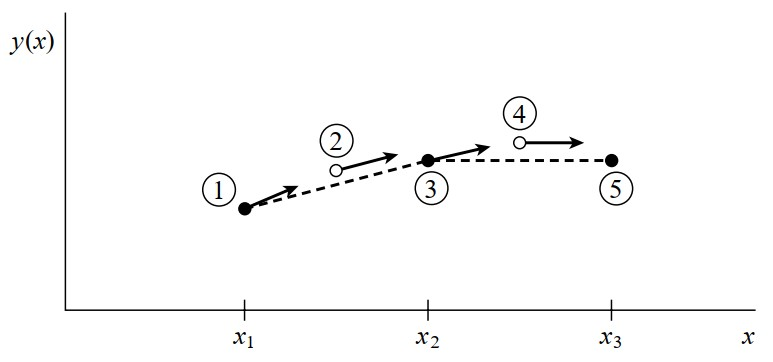
\includegraphics[width=\columnwidth]{Images/rk4.jpg}
    \caption{Schematic representation of the time integration of the Runge Kutta 4 (extracted from \cite{numerical_recipes})}
    \label{fig:rk4}
\end{figure}

When working with non-linear systems of equations like nonlinear wave equations and all the Einstein equations, many numerical methods may be susceptible to explosive growth of the error because of the effects of coefficients that depend on dynamical variables and because of lower-order terms. In order to solve these problems, we can add dissipative terms to the finite difference operators to dampen these effects and make our solution stable. \cite{book}

The standard way of adding artificial dissipation to a finite difference approximation is known as Kreiss-Oliger Dissipation, which the general formula for this kind of dissipation for a scheme with accuracy $2r-2$ is 

\begin{align}
    Q = \sigma (-1)^{r-1} h^{2r-1}(D_+)^r \rho (D_-)^r /2^{2r},
    \label{eq:dissipation_general}
\end{align}

\noindent
where $D_+$ and $D_-$ are the forward and backward finite difference operators respectively,  $\sigma$ regulates the strength of the dissipation and $\rho$ is a weighting function typically set to $1$ in the interior but may go to $0$ at the boundary.\cite{article}


\subsection{Convergence of a Numerical Method}
A numerical calculation done at one single resolution is meaningless. We must study how our solution behaves as we increase resolution. Since numerical calculations are nothing but approximations of the differential equations we are trying to solve, we need some way to measure the error in that approximation. For that purpose, we do what is called a \textit{convergence test}.

The solution of a stable finite difference approximation can be interpreted as the expansion of a continuum function in a power series with a discretization parameter $\Delta$, 

\begin{align}
    u_\Delta (t,x) = u(t,x) + \sum_{i=1}^{\infty} \Delta^i e_i (t,x),
    \label{eq:discrete_error}
\end{align}

\noindent
where $u(t,x)$ is the solution of the original differential equation and $e_i$ are the approximation error functions of order $i$. \cite{book}



In order to test the convergence of our numerical method, we can do what is called a \textit{norm convergence test}. To do this, we calculate the solution for our equation with three different resolutions ($\Delta1 >\Delta2 > \Delta3$) and compare their relative errors by defining a \textit{convergence factor} 

\begin{align}
    c(t) = \frac{||u_{\Delta_1} - u_{\Delta_2}||}{||u_{\Delta_2} - u_{\Delta_3}||},
    \label{eq:norm_convergence}
\end{align}

\noindent
where the differences must be taken in coinciding points. In this project, the $L^2$ norm was used, which is defined in equation for cartesian coordinates as 

\begin{align}
    ||u||(t) = \sqrt{\Delta x \sum_{x} (u(t,x))^2},
    \label{eq:norm_cartesian}
\end{align}

\noindent
and for spherical coordinates is defined as

\begin{align}
    ||u||(t) = \sqrt{4 \pi \Delta r \sum_{r} r^2(u(t,r))^2}.
    \label{eq:norm_spherical}
\end{align}

By taking $\Delta_1$, $\Delta_2$ and $\Delta_3$ such that $\Delta_1 / \Delta_2 = \Delta_2 / \Delta_3 = r$, we expect that our approximation in the continuum limit behaves as 

\begin{align}
    \lim_{\Delta \to 0} c(t) = \frac{\Delta_1^n - \Delta_2^n}{\Delta_2^n - \Delta_3^n} = r^n.
    \label{eq:norm_convergence_limit}
\end{align}

If we know the analytical solution for our equation, we can substitute the solution with resolution $\Delta_2$ with the analytical solution and perform the same test.

We can also calculate the relative errors $u_{\Delta_1} - u_{\Delta_2}$ and $u_{\Delta_2} - u_{\Delta_3}$ locally and compare them visually, doing what's called a \textit{pointwise convergence test}. According to the series expansion in equation \eqref{eq:discrete_error}, each error will be proportional to $e_i$. This way, if we scale the relative errors accordingly, they should all lay on top of each other.